\subsection{Examples}
\begin{namedframe}{Odd Number Squared}
	\begin{example}
		Given an odd integer $N$, prove that $N^2$ is also an odd integer.	
	\end{example}
	\pause
	If $N$ is odd, it can be expressed as $2M-1$.
	\pause
	\begin{align*}
		\uncover<+->{N^2 &= (2M-1)^2\\}
		\uncover<+->{ &= 4M^2-2M+1\\}
		\uncover<+->{ &= 2(2M^2-M)+1}
	\end{align*}
	\uncover<+->{
	Therefore $N^2$ is also odd.}	
\end{namedframe}
\begin{namedframe}{Pythagorean Theorem}
	\begin{example}
		Given a right angled triangle, the sum of the squares of the two legs is equal to the square of the hypotenuse.	
	\end{example}
	\begin{column}{0.5\textwidth}
	\begin{tikzpicture}[scale = 0.5]
		\coordinate [label=below left:$A$](A) at (0,0);
		\coordinate [label=below right:$B$](B) at (4,0);
		\coordinate [label=above right:$C$](C) at (4,3);
		
		\draw (A) -- (B) -- (C) -- cycle;
		\draw (A) rectangle (4,-4)node [midway] {$b^2$};
		\draw (B) rectangle (7,3)node [midway] {$a^2$};
		\draw [rotate around={36.8:(A)}](A) rectangle (5,5) node [midway] {$c^2$};
	\end{tikzpicture}
	\end{column}
	\pause
	\begin{column}{0.5\textwidth}
		In Canada, this theorem is provided to students without proof, despite the fact that over 1000 different ones exist.
	\end{column}
\end{namedframe}
\begin{namedframe}{Pythagorean Theorem}
	\pause
	\begin{column}{0.5\textwidth}
		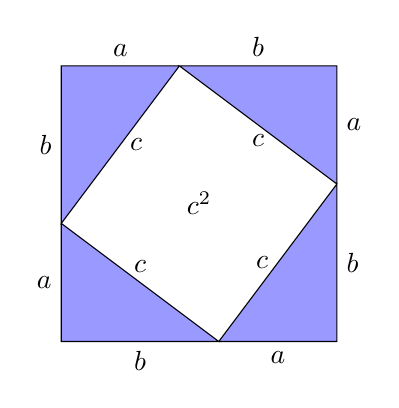
\begin{tikzpicture}[scale = 0.5]
		\coordinate (A) at (0,0);
		\coordinate (B) at (7,0);
		\coordinate (C) at (7,7);
		\coordinate (D) at (0,7);
		\coordinate (AB) at (4,0);
		\coordinate (BC) at (7,4);
		\coordinate (CD) at (3,7);
		\coordinate (DA) at (0,3);

		%\draw (A)rectangle(C) node [midway] {$c^2$};
		%\draw (A) -- node[below]{$b$}(AB) -- node[below]{$a$}(B);
		%\draw (B) -- node[right]{$b$}(BC) -- node[right]{$a$}(C);
		%\draw (C) -- node[above]{$b$}(CD) -- node[above]{$a$}(D);
		%\draw (D) -- node[left]{$b$}(DA) -- node[left]{$a$}(A);
		%\draw (AB) -- node[left]{$c$}(BC) -- node[below]{$c$}(CD) -- node[right]{$c$}(DA) -- node[above]{$c$}(AB) ; 
		\draw (3.5,3.5)node {$c^2$};
		
		\filldraw[fill=blue!40!white, draw=black] (DA) -- node[left]{$a$}(A) -- node[below]{$b$}(AB) -- node[above]{$c$}(DA);
		\filldraw[fill=blue!40!white, draw=black] (AB) -- node[below]{$a$}(B) -- node[right]{$b$}(BC) -- node[left]{$c$}(AB);
		\filldraw[fill=blue!40!white, draw=black] (BC) -- node[right]{$a$}(C) -- node[above]{$b$}(CD) -- node[below]{$c$}(BC);
		\filldraw[fill=blue!40!white, draw=black] (CD) -- node[above]{$a$}(D) -- node[left]{$b$}(DA) -- node[right]{$c$}(CD);
		\end{tikzpicture}
	\end{column}
	\pause
	\begin{column}{0.5\textwidth}
		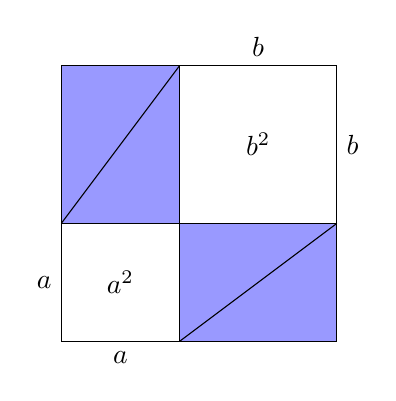
\begin{tikzpicture}[scale = 0.5]
		\coordinate (A) at (0,0);
		\coordinate (B) at (7,0);
		\coordinate (C) at (7,7);
		\coordinate (D) at (0,7);
		\coordinate (AB) at (3,0);
		\coordinate (BC) at (7,3);
		\coordinate (CD) at (3,7);
		\coordinate (DA) at (0,3);
		
		\filldraw[fill=blue!40!white, draw=black]  (AB) rectangle (BC);
		\filldraw[fill=blue!40!white, draw=black]  (CD) rectangle (DA);
		\draw (AB) -- (BC);
		\draw (CD) -- (DA);
		\draw (DA) -- node[left]{$a$}(A) -- node[below]{$a$}(AB);
		\draw (BC) -- node[right]{$b$}(C) -- node[above]{$b$}(CD);
		
		\draw (1.5,1.5)node {$a^2$};
		\draw (5,5)node {$b^2$};
		%\filldraw[fill=blue!40!white, draw=black]  (CD) -- (D) -- (DA) -- (CD);
		%\filldraw[fill=blue!40!white, draw=black]  (AB) -- (B) -- (BC) -- (AB);
		\end{tikzpicture}
	\end{column}
\end{namedframe}